\section{Дополнительный модуль ut1, подключаемый к учебной программе}



%---------------------------------------------------------
%Two columns
\begin{frame}
\frametitle{Дополнительные возможности для учебных программ}

\begin{itemize}
\item В задачнике Programming Taskbook для получения исходных и вывода результирующих данных предусмотрены специальные функции, связывающие учебную программу и ядро задачника.
\item В первой версии задачника Unix Taskbook использование особых функций ввода-вывода не было предусмотрено. В ранее разработанных группах заданий исходные данные передаются через механизм параметров командной строки, а результаты записываются (или перенаправляются) в файл, который анализируется задачником.
\end{itemize}

\end{frame}
%---------------------------------------------------------


%---------------------------------------------------------
%Two columns
\begin{frame}
\frametitle{Реализация вспомогательного модуля для учебной программы}
\begin{block}{Задача}
предусмотреть в задачнике Unix Taskbook возможность использования специальных средств ввода-вывода для задач, импортированных из задачника Programming Taskbook.
\end{block}

\begin{block}{Решение}
    разработать \textbf{вспомогательный подключаемый модуль} с функциями, которые позволяют получать исходные данные, подготовленные задачником, и передавать ему найденные результаты.
\end{block}


\end{frame}
%---------------------------------------------------------


%---------------------------------------------------------
%Highlighting text
\begin{frame}
\frametitle{Особенности подключаемого модуля ut1mpi.c и ut1.c}


\begin{itemize}
\item Реализован на языке C, включает все функции ввода, вывода и отладки, имеющиеся в задачнике Programming Taskbook.
\item Может использоваться как для программы, запускаемой под управлением задачника Unix Taskbook, так и для независимой программы (консольного приложения).
\begin{itemize}
    \item В случае использования задачника исходные данные считываются из специальных файлов ввода, результаты и отладочные данные также сохраняются в специальных файлах вывода и отладки и затем анализируются и отображаются на экране средствами задачника.
    \item В случае обычного консольного приложения исходные данные должны вводиться с клавиатуры, а результаты и отладочные данные выводятся на экран.
\end{itemize}
\end{itemize}


\end{frame}
%---------------------------------------------------------


%---------------------------------------------------------
%Two columns
\begin{frame}
\frametitle{Особенности подключаемого модуля ut1mpi.c и ut1.c}

\begin{columns}
\column{0.5\textwidth}
\begin{figure}[htbp]%
    \centering
    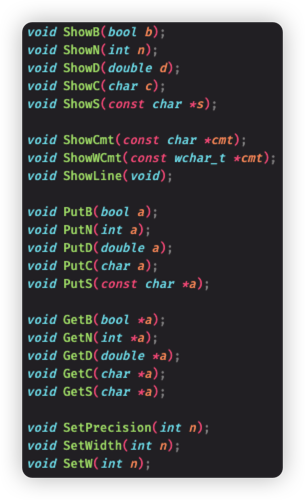
\includegraphics[width=0.6\linewidth]{images/ut1.jpg}%子图文件名
    \caption{ut1.h}%总标题
    \label{ut1}%总标签
\end{figure}

\column{0.5\textwidth}
\begin{figure}[htbp]%
    \centering
    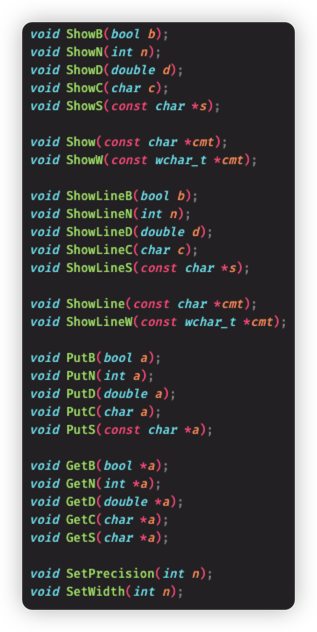
\includegraphics[width=0.5\linewidth]{images/ut1mpi.jpg}%子图文件名
    \caption{ut1.h for mpi}%总标题
    \label{ut1mpi}%总标签
\end{figure}
\end{columns}

\end{frame}
%---------------------------------------------------------


%---------------------------------------------------------
%Highlighting text
\begin{frame}
\frametitle{Новый вариант подсистемы проверки для Unix Taskbook}

\begin{block}{Прежний вариант}
    нализировалось содержимое файла, созданного учебной программой (или полученного в результате перенаправления стандартного потока вывода для учебной программы).
\end{block}

\begin{block}{Новый вариант}
анализируется содержимое \textbf{специальных файлов}, генерируемых подключаемым модулем ut1. Дополнительно выявляются \textbf{различные виды ошибок ввода-вывода}.
\end{block}

% \begin{itemize}
% \item Прежний вариант: анализировалось содержимое файла, созданного учебной программой (или полученного в результате перенаправления стандартного потока вывода для учебной программы).
% \item Новый вариант: анализируется содержимое \textbf{специальных файлов}, генерируемых подключаемым модулем ut1. Дополнительно выявляются \textbf{различные виды ошибок ввода-вывода}.
% \end{itemize}


\end{frame}
%---------------------------------------------------------